% Options for packages loaded elsewhere
\PassOptionsToPackage{unicode}{hyperref}
\PassOptionsToPackage{hyphens}{url}
\PassOptionsToPackage{dvipsnames,svgnames,x11names}{xcolor}
%
\documentclass[
  letterpaper,
  DIV=11,
  numbers=noendperiod]{scrartcl}

\usepackage{amsmath,amssymb}
\usepackage{iftex}
\ifPDFTeX
  \usepackage[T1]{fontenc}
  \usepackage[utf8]{inputenc}
  \usepackage{textcomp} % provide euro and other symbols
\else % if luatex or xetex
  \usepackage{unicode-math}
  \defaultfontfeatures{Scale=MatchLowercase}
  \defaultfontfeatures[\rmfamily]{Ligatures=TeX,Scale=1}
\fi
\usepackage{lmodern}
\ifPDFTeX\else  
    % xetex/luatex font selection
\fi
% Use upquote if available, for straight quotes in verbatim environments
\IfFileExists{upquote.sty}{\usepackage{upquote}}{}
\IfFileExists{microtype.sty}{% use microtype if available
  \usepackage[]{microtype}
  \UseMicrotypeSet[protrusion]{basicmath} % disable protrusion for tt fonts
}{}
\makeatletter
\@ifundefined{KOMAClassName}{% if non-KOMA class
  \IfFileExists{parskip.sty}{%
    \usepackage{parskip}
  }{% else
    \setlength{\parindent}{0pt}
    \setlength{\parskip}{6pt plus 2pt minus 1pt}}
}{% if KOMA class
  \KOMAoptions{parskip=half}}
\makeatother
\usepackage{xcolor}
\setlength{\emergencystretch}{3em} % prevent overfull lines
\setcounter{secnumdepth}{-\maxdimen} % remove section numbering
% Make \paragraph and \subparagraph free-standing
\makeatletter
\ifx\paragraph\undefined\else
  \let\oldparagraph\paragraph
  \renewcommand{\paragraph}{
    \@ifstar
      \xxxParagraphStar
      \xxxParagraphNoStar
  }
  \newcommand{\xxxParagraphStar}[1]{\oldparagraph*{#1}\mbox{}}
  \newcommand{\xxxParagraphNoStar}[1]{\oldparagraph{#1}\mbox{}}
\fi
\ifx\subparagraph\undefined\else
  \let\oldsubparagraph\subparagraph
  \renewcommand{\subparagraph}{
    \@ifstar
      \xxxSubParagraphStar
      \xxxSubParagraphNoStar
  }
  \newcommand{\xxxSubParagraphStar}[1]{\oldsubparagraph*{#1}\mbox{}}
  \newcommand{\xxxSubParagraphNoStar}[1]{\oldsubparagraph{#1}\mbox{}}
\fi
\makeatother

\usepackage{color}
\usepackage{fancyvrb}
\newcommand{\VerbBar}{|}
\newcommand{\VERB}{\Verb[commandchars=\\\{\}]}
\DefineVerbatimEnvironment{Highlighting}{Verbatim}{commandchars=\\\{\}}
% Add ',fontsize=\small' for more characters per line
\usepackage{framed}
\definecolor{shadecolor}{RGB}{241,243,245}
\newenvironment{Shaded}{\begin{snugshade}}{\end{snugshade}}
\newcommand{\AlertTok}[1]{\textcolor[rgb]{0.68,0.00,0.00}{#1}}
\newcommand{\AnnotationTok}[1]{\textcolor[rgb]{0.37,0.37,0.37}{#1}}
\newcommand{\AttributeTok}[1]{\textcolor[rgb]{0.40,0.45,0.13}{#1}}
\newcommand{\BaseNTok}[1]{\textcolor[rgb]{0.68,0.00,0.00}{#1}}
\newcommand{\BuiltInTok}[1]{\textcolor[rgb]{0.00,0.23,0.31}{#1}}
\newcommand{\CharTok}[1]{\textcolor[rgb]{0.13,0.47,0.30}{#1}}
\newcommand{\CommentTok}[1]{\textcolor[rgb]{0.37,0.37,0.37}{#1}}
\newcommand{\CommentVarTok}[1]{\textcolor[rgb]{0.37,0.37,0.37}{\textit{#1}}}
\newcommand{\ConstantTok}[1]{\textcolor[rgb]{0.56,0.35,0.01}{#1}}
\newcommand{\ControlFlowTok}[1]{\textcolor[rgb]{0.00,0.23,0.31}{\textbf{#1}}}
\newcommand{\DataTypeTok}[1]{\textcolor[rgb]{0.68,0.00,0.00}{#1}}
\newcommand{\DecValTok}[1]{\textcolor[rgb]{0.68,0.00,0.00}{#1}}
\newcommand{\DocumentationTok}[1]{\textcolor[rgb]{0.37,0.37,0.37}{\textit{#1}}}
\newcommand{\ErrorTok}[1]{\textcolor[rgb]{0.68,0.00,0.00}{#1}}
\newcommand{\ExtensionTok}[1]{\textcolor[rgb]{0.00,0.23,0.31}{#1}}
\newcommand{\FloatTok}[1]{\textcolor[rgb]{0.68,0.00,0.00}{#1}}
\newcommand{\FunctionTok}[1]{\textcolor[rgb]{0.28,0.35,0.67}{#1}}
\newcommand{\ImportTok}[1]{\textcolor[rgb]{0.00,0.46,0.62}{#1}}
\newcommand{\InformationTok}[1]{\textcolor[rgb]{0.37,0.37,0.37}{#1}}
\newcommand{\KeywordTok}[1]{\textcolor[rgb]{0.00,0.23,0.31}{\textbf{#1}}}
\newcommand{\NormalTok}[1]{\textcolor[rgb]{0.00,0.23,0.31}{#1}}
\newcommand{\OperatorTok}[1]{\textcolor[rgb]{0.37,0.37,0.37}{#1}}
\newcommand{\OtherTok}[1]{\textcolor[rgb]{0.00,0.23,0.31}{#1}}
\newcommand{\PreprocessorTok}[1]{\textcolor[rgb]{0.68,0.00,0.00}{#1}}
\newcommand{\RegionMarkerTok}[1]{\textcolor[rgb]{0.00,0.23,0.31}{#1}}
\newcommand{\SpecialCharTok}[1]{\textcolor[rgb]{0.37,0.37,0.37}{#1}}
\newcommand{\SpecialStringTok}[1]{\textcolor[rgb]{0.13,0.47,0.30}{#1}}
\newcommand{\StringTok}[1]{\textcolor[rgb]{0.13,0.47,0.30}{#1}}
\newcommand{\VariableTok}[1]{\textcolor[rgb]{0.07,0.07,0.07}{#1}}
\newcommand{\VerbatimStringTok}[1]{\textcolor[rgb]{0.13,0.47,0.30}{#1}}
\newcommand{\WarningTok}[1]{\textcolor[rgb]{0.37,0.37,0.37}{\textit{#1}}}

\providecommand{\tightlist}{%
  \setlength{\itemsep}{0pt}\setlength{\parskip}{0pt}}\usepackage{longtable,booktabs,array}
\usepackage{calc} % for calculating minipage widths
% Correct order of tables after \paragraph or \subparagraph
\usepackage{etoolbox}
\makeatletter
\patchcmd\longtable{\par}{\if@noskipsec\mbox{}\fi\par}{}{}
\makeatother
% Allow footnotes in longtable head/foot
\IfFileExists{footnotehyper.sty}{\usepackage{footnotehyper}}{\usepackage{footnote}}
\makesavenoteenv{longtable}
\usepackage{graphicx}
\makeatletter
\newsavebox\pandoc@box
\newcommand*\pandocbounded[1]{% scales image to fit in text height/width
  \sbox\pandoc@box{#1}%
  \Gscale@div\@tempa{\textheight}{\dimexpr\ht\pandoc@box+\dp\pandoc@box\relax}%
  \Gscale@div\@tempb{\linewidth}{\wd\pandoc@box}%
  \ifdim\@tempb\p@<\@tempa\p@\let\@tempa\@tempb\fi% select the smaller of both
  \ifdim\@tempa\p@<\p@\scalebox{\@tempa}{\usebox\pandoc@box}%
  \else\usebox{\pandoc@box}%
  \fi%
}
% Set default figure placement to htbp
\def\fps@figure{htbp}
\makeatother
% definitions for citeproc citations
\NewDocumentCommand\citeproctext{}{}
\NewDocumentCommand\citeproc{mm}{%
  \begingroup\def\citeproctext{#2}\cite{#1}\endgroup}
\makeatletter
 % allow citations to break across lines
 \let\@cite@ofmt\@firstofone
 % avoid brackets around text for \cite:
 \def\@biblabel#1{}
 \def\@cite#1#2{{#1\if@tempswa , #2\fi}}
\makeatother
\newlength{\cslhangindent}
\setlength{\cslhangindent}{1.5em}
\newlength{\csllabelwidth}
\setlength{\csllabelwidth}{3em}
\newenvironment{CSLReferences}[2] % #1 hanging-indent, #2 entry-spacing
 {\begin{list}{}{%
  \setlength{\itemindent}{0pt}
  \setlength{\leftmargin}{0pt}
  \setlength{\parsep}{0pt}
  % turn on hanging indent if param 1 is 1
  \ifodd #1
   \setlength{\leftmargin}{\cslhangindent}
   \setlength{\itemindent}{-1\cslhangindent}
  \fi
  % set entry spacing
  \setlength{\itemsep}{#2\baselineskip}}}
 {\end{list}}
\usepackage{calc}
\newcommand{\CSLBlock}[1]{\hfill\break\parbox[t]{\linewidth}{\strut\ignorespaces#1\strut}}
\newcommand{\CSLLeftMargin}[1]{\parbox[t]{\csllabelwidth}{\strut#1\strut}}
\newcommand{\CSLRightInline}[1]{\parbox[t]{\linewidth - \csllabelwidth}{\strut#1\strut}}
\newcommand{\CSLIndent}[1]{\hspace{\cslhangindent}#1}

\KOMAoption{captions}{tableheading}
\makeatletter
\@ifpackageloaded{caption}{}{\usepackage{caption}}
\AtBeginDocument{%
\ifdefined\contentsname
  \renewcommand*\contentsname{Table of contents}
\else
  \newcommand\contentsname{Table of contents}
\fi
\ifdefined\listfigurename
  \renewcommand*\listfigurename{List of Figures}
\else
  \newcommand\listfigurename{List of Figures}
\fi
\ifdefined\listtablename
  \renewcommand*\listtablename{List of Tables}
\else
  \newcommand\listtablename{List of Tables}
\fi
\ifdefined\figurename
  \renewcommand*\figurename{Figure}
\else
  \newcommand\figurename{Figure}
\fi
\ifdefined\tablename
  \renewcommand*\tablename{Table}
\else
  \newcommand\tablename{Table}
\fi
}
\@ifpackageloaded{float}{}{\usepackage{float}}
\floatstyle{ruled}
\@ifundefined{c@chapter}{\newfloat{codelisting}{h}{lop}}{\newfloat{codelisting}{h}{lop}[chapter]}
\floatname{codelisting}{Listing}
\newcommand*\listoflistings{\listof{codelisting}{List of Listings}}
\makeatother
\makeatletter
\makeatother
\makeatletter
\@ifpackageloaded{caption}{}{\usepackage{caption}}
\@ifpackageloaded{subcaption}{}{\usepackage{subcaption}}
\makeatother

\usepackage{bookmark}

\IfFileExists{xurl.sty}{\usepackage{xurl}}{} % add URL line breaks if available
\urlstyle{same} % disable monospaced font for URLs
\hypersetup{
  pdftitle={Final Project: Data Ethics and Policy},
  colorlinks=true,
  linkcolor={blue},
  filecolor={Maroon},
  citecolor={Blue},
  urlcolor={Blue},
  pdfcreator={LaTeX via pandoc}}


\title{Final Project: Data Ethics and Policy}
\author{Christy Hsu}
\date{}

\begin{document}
\maketitle


\subsection{Abstract}\label{abstract}

This project looked into an attempt in the fifties that set out to
measure individual tolerance and use that measure to evaluate the impact
the anti-Communism Cold War agenda---both abroad and at home---had on
U.S. citizens. I saw the picking up of this 70-year-old survey data, and
the analysis that accompanied it, as a chance to stroll through the data
ethics concerns that can arise when holding the hope to learn about the
world from data

\subsection{Introduction}\label{introduction}

The online poll data library host by Roper Center was where I first came
across the Stouffer Study of 1954 \emph{Communism, Conformity, and Civil
Liberties: A Cross-Section of the Nation Speaks Its Mind} by Samuel
Andrew
Stouffer(\citeproc{ref-fundfortherepublicCommunismConformityAmp2020}{Fund
For The Republic and Stouffer 2020})And, I gained access to the entire
dataset on
ICPSR(\citeproc{ref-stoufferCommunismConformityCivil1992}{Samuel A.
Stouffer 1992})


\includegraphics[width=0.5\linewidth,height=\textheight,keepaspectratio]{image/stouffer-cover.png}

I found Stouffer's attempt in the fifties to design public opion polls
and, construct an innovative way of measuring the latent properties
tolerance and fear at the individual level very interesting. The
tolerance scale and the perception of internal communist danger scale
are not included in the data, thus a major part of this project involved
returning these two target variables in order to complete the picture
and reproduce that basis on which Stouffer built his arguments. I
learned much from this practice of reading and researching that past
effort into conceptualizing and operationalizing tolerance and fear, and
got my hands dirty to really apply those framings and methods to the
data. It gave me a chance to reflect on the many artistic and arbitrary
decisions that the researcher made throughout this data analysis
process.

\textsubscript{Source:
\href{https://h-christy.github.io/data-ethics-final/index.qmd.html}{Article
Notebook}}

\textsubscript{Source:
\href{https://h-christy.github.io/data-ethics-final/index.qmd.html}{Article
Notebook}}

\subsection{Harvesting from Historical Data Collection Efforts: A More
Friendly
Format}\label{harvesting-from-historical-data-collection-efforts-a-more-friendly-format}

Complying ICPSR's redistribution policy, the converted data files are
not provided here. Instead, the author provides STATA .do and .dct
files, which were constructed based on the reading of the codebook.
Please down the the dataset in ASCII format from ICPSR and should be
able to apply to decode the .txt files from both
samples.(\citeproc{ref-stoufferCommunismConformityCivil1992}{Samuel A.
Stouffer 1992})

\begin{verbatim}
├── read-ascii-files
│   ├── gp-decode.do
│   ├── lead-decode.do
│   ├── sample1.dct
│   └── sample2.dct
\end{verbatim}

\subsection{Returning target variables to the
data}\label{returning-target-variables-to-the-data}

The tolerance that Stouffer argued
upon.(\citeproc{ref-stouffer1955communism}{Samuel Andrew Stouffer 1955,
262--69})

\paragraph{\texorpdfstring{Preparing the \texttt{code\_df} data
frame}{Preparing the code\_df data frame}}\label{preparing-the-code_df-data-frame}

\begin{enumerate}
\def\labelenumi{\arabic{enumi}.}
\tightlist
\item
  Cleaning column names and binding the two samples
\end{enumerate}

\textsubscript{Source:
\href{https://h-christy.github.io/data-ethics-final/index.qmd.html}{Article
Notebook}}

\textsubscript{Source:
\href{https://h-christy.github.io/data-ethics-final/index.qmd.html}{Article
Notebook}}

\paragraph{\texorpdfstring{Adding Binary and Ternary Variables
\texttt{leader},\texttt{interested} and \texttt{categorizer}: these are
the variables that Stouffer specified in his book as ways to divide the
respondents and make
comparisons.}{Adding Binary and Ternary Variables leader,interested and categorizer: these are the variables that Stouffer specified in his book as ways to divide the respondents and make comparisons.}}\label{adding-binary-and-ternary-variables-leaderinterested-and-categorizer-these-are-the-variables-that-stouffer-specified-in-his-book-as-ways-to-divide-the-respondents-and-make-comparisons.}

\begin{longtable}[]{@{}rr@{}}
\toprule\noalign{}
leader & n \\
\midrule\noalign{}
\endhead
\bottomrule\noalign{}
\endlastfoot
0 & 4933 \\
1 & 1500 \\
\end{longtable}

\textsubscript{Source:
\href{https://h-christy.github.io/data-ethics-final/index.qmd.html}{Article
Notebook}}

\begin{longtable}[]{@{}rlrr@{}}
\toprule\noalign{}
leader & interested & n & pct \\
\midrule\noalign{}
\endhead
\bottomrule\noalign{}
\endlastfoot
0 & less & 2155 & 43.68538 \\
0 & more & 2778 & 56.31462 \\
1 & less & 210 & 14.00000 \\
1 & more & 1290 & 86.00000 \\
\end{longtable}

\textsubscript{Source:
\href{https://h-christy.github.io/data-ethics-final/index.qmd.html}{Article
Notebook}}

\textsubscript{Source:
\href{https://h-christy.github.io/data-ethics-final/index.qmd.html}{Article
Notebook}}

\begin{longtable}[]{@{}rlrr@{}}
\toprule\noalign{}
leader & categorizer & n & pct \\
\midrule\noalign{}
\endhead
\bottomrule\noalign{}
\endlastfoot
0 & agree & 3127 & 63.389418 \\
0 & disagree & 1495 & 30.306102 \\
0 & dont know & 311 & 6.304480 \\
1 & agree & 806 & 53.733333 \\
1 & disagree & 669 & 44.600000 \\
1 & dont know & 25 & 1.666667 \\
\end{longtable}

\textsubscript{Source:
\href{https://h-christy.github.io/data-ethics-final/index.qmd.html}{Article
Notebook}}

\subsection{Scale1: Willingness to Tolerate
Nonconformist}\label{scale1-willingness-to-tolerate-nonconformist}

\paragraph{Conceptual Tolerance and Operational
Tolerance}\label{conceptual-tolerance-and-operational-tolerance}

The questionnaires used to rank respondents into six tolerance groups
focused on four types of nonconformists:

\begin{itemize}
\tightlist
\item
  A person who is against all churches and religion (atheist)
\item
  A person who favors government ownership (socialist)
\item
  An alleged communist (someone whose loyalty has been questioned by a
  Congressional Committee but swears under oath they have never been a
  communist)
\item
  An admitted communist
\end{itemize}

respondent were asked about their approval of 3 types of disposition
against the above nonconfromist, and whether they agree or disagree the
limitation or deprivation of the nonconformist's civil liberties, for
example:

\begin{enumerate}
\def\labelenumi{\arabic{enumi}.}
\item
  Freedom speech:

  \begin{itemize}
  \tightlist
  \item
    ``If \_\_\_ wants to make a speech in your community, should he be
    allowed to speak or not?''
  \end{itemize}
\item
  Book censor:

  \begin{itemize}
  \tightlist
  \item
    ``Suppose he wrote a book that is in your public library. Somebody
    in your community suggests the book should be removed. Would you
    favor removing it, or not?''
  \end{itemize}
\item
  Employment:

  \begin{itemize}
  \tightlist
  \item
    Should a radio singer who is a nonconformist be fired or not?
  \item
    Should a college or university teacher be fired or not?
  \item
    Should a high school teacher be fired or not?
  \item
    Should someone working in a defense plant be fired or not?
  \item
    Should a store clerk be fired or not?
  \end{itemize}
\item
  Boycott:

  \begin{itemize}
  \tightlist
  \item
    ``Suppose the radio program he is on advertises a brand of soap.
    Somebody in your community suggests you stop buying that soap. Would
    you stop or not?''
  \end{itemize}
\end{enumerate}

\paragraph{0 to 5: Scaling Individual
Tolerance}\label{to-5-scaling-individual-tolerance}

I ran into many challenges replicating Stouffer's results. Both the
overall proportions across tolerance rankings, was unable to reproduce
the group counts applying further breakdowns, such as by age, region,
education, thus for comparison.

\textsubscript{Source:
\href{https://h-christy.github.io/data-ethics-final/index.qmd.html}{Article
Notebook}}

\textsubscript{Source:
\href{https://h-christy.github.io/data-ethics-final/index.qmd.html}{Article
Notebook}}

\textsubscript{Source:
\href{https://h-christy.github.io/data-ethics-final/index.qmd.html}{Article
Notebook}}

\textsubscript{Source:
\href{https://h-christy.github.io/data-ethics-final/index.qmd.html}{Article
Notebook}}

\textsubscript{Source:
\href{https://h-christy.github.io/data-ethics-final/index.qmd.html}{Article
Notebook}}

\begin{longtable}[]{@{}rlrr@{}}
\toprule\noalign{}
leader & tolerance\_group & n & pct \\
\midrule\noalign{}
\endhead
\bottomrule\noalign{}
\endlastfoot
0 & tolerance0 & 651 & 13.196838 \\
0 & tolerance1 & 871 & 17.656598 \\
0 & tolerance2 & 1263 & 25.603081 \\
0 & tolerance3 & 951 & 19.278330 \\
0 & tolerance4 & 395 & 8.007298 \\
0 & tolerance5 & 802 & 16.257855 \\
1 & tolerance0 & 79 & 5.266667 \\
1 & tolerance1 & 182 & 12.133333 \\
1 & tolerance2 & 180 & 12.000000 \\
1 & tolerance3 & 246 & 16.400000 \\
1 & tolerance4 & 205 & 13.666667 \\
1 & tolerance5 & 608 & 40.533333 \\
\end{longtable}

\textsubscript{Source:
\href{https://h-christy.github.io/data-ethics-final/index.qmd.html}{Article
Notebook}}

\begin{longtable}[]{@{}lr@{}}
\toprule\noalign{}
tolerance\_group & n \\
\midrule\noalign{}
\endhead
\bottomrule\noalign{}
\endlastfoot
tolerance0 & 730 \\
tolerance1 & 1053 \\
tolerance2 & 1443 \\
tolerance3 & 1197 \\
tolerance4 & 600 \\
tolerance5 & 1410 \\
\end{longtable}

\textsubscript{Source:
\href{https://h-christy.github.io/data-ethics-final/index.qmd.html}{Article
Notebook}}

\paragraph{\texorpdfstring{Broader Tolerance Rank Groups:
\texttt{less\ tolerant}, \texttt{in-between} and
\texttt{more\ tolerant}}{Broader Tolerance Rank Groups: less tolerant, in-between and more tolerant}}\label{broader-tolerance-rank-groups-less-tolerant-in-between-and-more-tolerant}

\textsubscript{Source:
\href{https://h-christy.github.io/data-ethics-final/index.qmd.html}{Article
Notebook}}

\begin{longtable}[]{@{}lrr@{}}
\toprule\noalign{}
tolerance\_broader0 & n & pct \\
\midrule\noalign{}
\endhead
\bottomrule\noalign{}
\endlastfoot
more tolerant & 813 & 54.2 \\
in between & 426 & 28.4 \\
less tolerant & 261 & 17.4 \\
\end{longtable}

\textsubscript{Source:
\href{https://h-christy.github.io/data-ethics-final/index.qmd.html}{Article
Notebook}}

\paragraph{Attempt2}\label{attempt2}

Allowing some inconsistency?

\textsubscript{Source:
\href{https://h-christy.github.io/data-ethics-final/index.qmd.html}{Article
Notebook}}

\begin{longtable}[]{@{}lr@{}}
\toprule\noalign{}
tolerance & n \\
\midrule\noalign{}
\endhead
\bottomrule\noalign{}
\endlastfoot
tolerance0 & 674 \\
tolerance1 & 530 \\
tolerance2 & 1334 \\
tolerance3 & 1229 \\
tolerance4 & 807 \\
tolerance5 & 1859 \\
\end{longtable}

\textsubscript{Source:
\href{https://h-christy.github.io/data-ethics-final/index.qmd.html}{Article
Notebook}}

\begin{longtable}[]{@{}rlrr@{}}
\toprule\noalign{}
leader & tolerance & n & pct \\
\midrule\noalign{}
\endhead
\bottomrule\noalign{}
\endlastfoot
0 & tolerance0 & 604 & 12.244070 \\
0 & tolerance1 & 491 & 9.953375 \\
0 & tolerance2 & 1179 & 23.900264 \\
0 & tolerance3 & 993 & 20.129738 \\
0 & tolerance4 & 554 & 11.230488 \\
0 & tolerance5 & 1112 & 22.542064 \\
1 & tolerance0 & 70 & 4.666667 \\
1 & tolerance1 & 39 & 2.600000 \\
1 & tolerance2 & 155 & 10.333333 \\
1 & tolerance3 & 236 & 15.733333 \\
1 & tolerance4 & 253 & 16.866667 \\
1 & tolerance5 & 747 & 49.800000 \\
\end{longtable}

\textsubscript{Source:
\href{https://h-christy.github.io/data-ethics-final/index.qmd.html}{Article
Notebook}}

\textsubscript{Source:
\href{https://h-christy.github.io/data-ethics-final/index.qmd.html}{Article
Notebook}}

\begin{longtable}[]{@{}rlrr@{}}
\toprule\noalign{}
leader & tolerance\_broader & n & pct \\
\midrule\noalign{}
\endhead
\bottomrule\noalign{}
\endlastfoot
0 & more tolerant & 1666 & 33.772552 \\
0 & in between & 2172 & 44.030002 \\
0 & less tolerant & 1095 & 22.197446 \\
1 & more tolerant & 1000 & 66.666667 \\
1 & in between & 391 & 26.066667 \\
1 & less tolerant & 109 & 7.266667 \\
\end{longtable}

\textsubscript{Source:
\href{https://h-christy.github.io/data-ethics-final/index.qmd.html}{Article
Notebook}}

To answer this question(\citeproc{ref-stouffer1955communism}{Samuel
Andrew Stouffer 1955, 51})

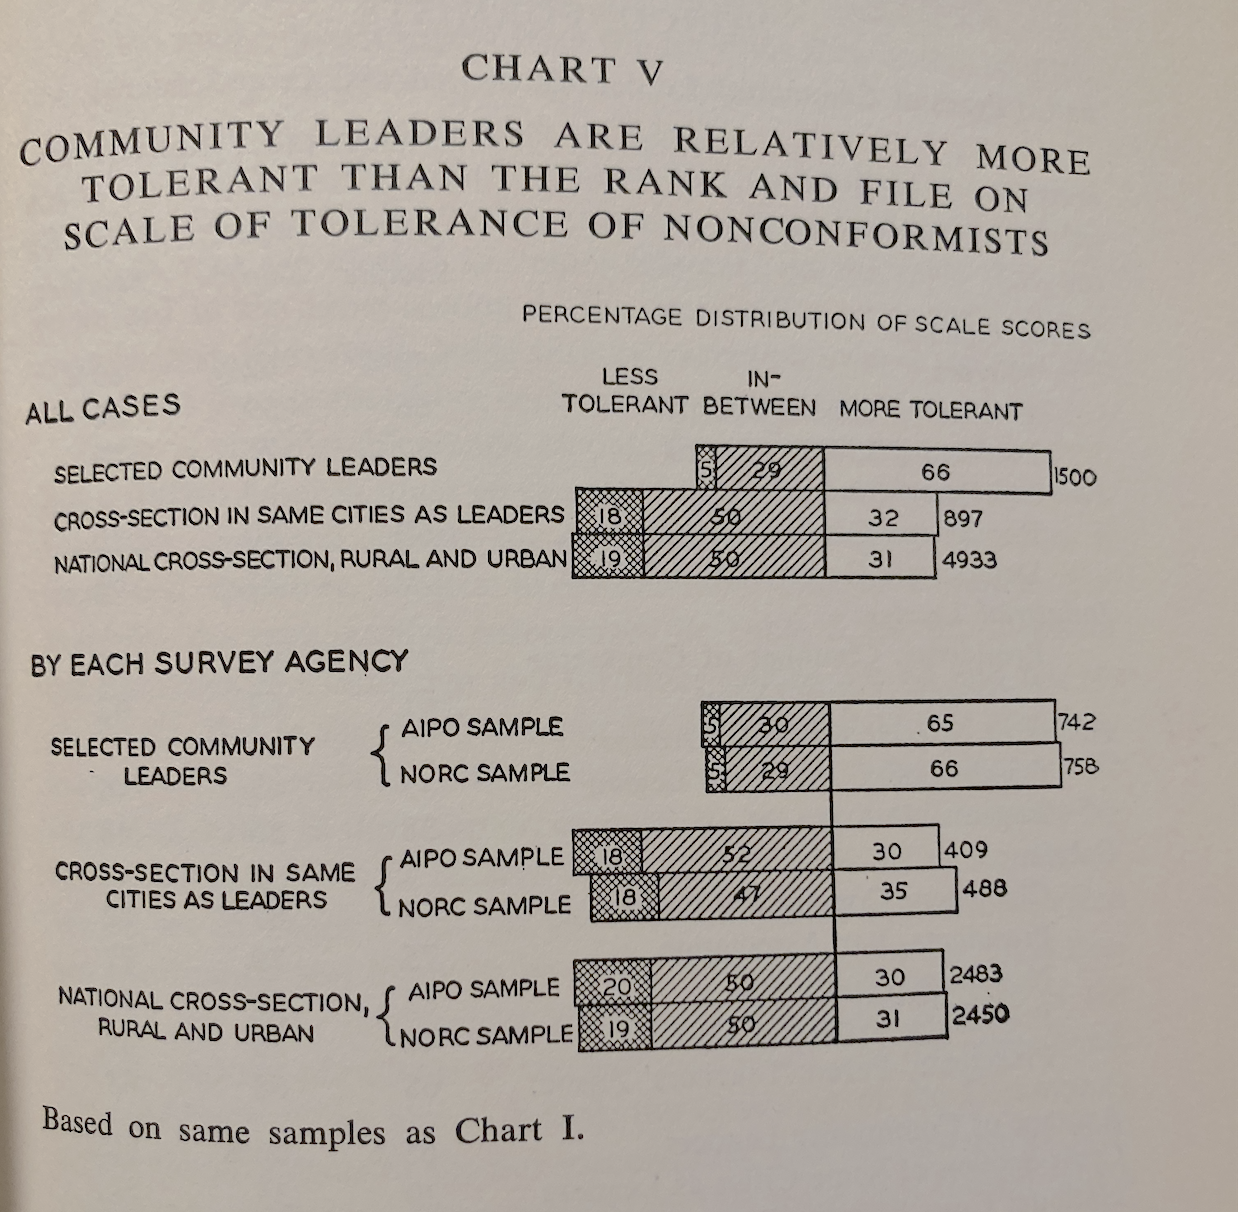
\includegraphics[width=0.5\linewidth,height=\textheight,keepaspectratio]{image/tolerance-distribution.png}

\subparagraph{us region}\label{us-region}

\textsubscript{Source:
\href{https://h-christy.github.io/data-ethics-final/index.qmd.html}{Article
Notebook}}

\begin{longtable}[]{@{}llrr@{}}
\toprule\noalign{}
us\_region & tolerance\_broader & n & pct \\
\midrule\noalign{}
\endhead
\bottomrule\noalign{}
\endlastfoot
east & more tolerant & 276 & 68.148148 \\
east & in between & 107 & 26.419753 \\
east & less tolerant & 22 & 5.432099 \\
midwest & more tolerant & 348 & 69.322709 \\
midwest & in between & 123 & 24.501992 \\
midwest & less tolerant & 31 & 6.175299 \\
south & more tolerant & 225 & 57.251908 \\
south & in between & 123 & 31.297710 \\
south & less tolerant & 45 & 11.450382 \\
west & more tolerant & 151 & 75.500000 \\
west & in between & 38 & 19.000000 \\
west & less tolerant & 11 & 5.500000 \\
\end{longtable}

\textsubscript{Source:
\href{https://h-christy.github.io/data-ethics-final/index.qmd.html}{Article
Notebook}}

\subsection{Scale2: Scale of the Perception on the Internal Communist
Danger}\label{scale2-scale-of-the-perception-on-the-internal-communist-danger}

\textsubscript{Source:
\href{https://h-christy.github.io/data-ethics-final/index.qmd.html}{Article
Notebook}}

\textsubscript{Source:
\href{https://h-christy.github.io/data-ethics-final/index.qmd.html}{Article
Notebook}}

\begin{longtable}[]{@{}lr@{}}
\toprule\noalign{}
danger & n \\
\midrule\noalign{}
\endhead
\bottomrule\noalign{}
\endlastfoot
danger0 & 507 \\
danger1 & 682 \\
danger2 & 2116 \\
danger3 & 1170 \\
danger4 & 1093 \\
danger5 & 865 \\
\end{longtable}

\textsubscript{Source:
\href{https://h-christy.github.io/data-ethics-final/index.qmd.html}{Article
Notebook}}

\subsubsection{Broader rank groups}\label{broader-rank-groups}

\textsubscript{Source:
\href{https://h-christy.github.io/data-ethics-final/index.qmd.html}{Article
Notebook}}

\begin{longtable}[]{@{}lr@{}}
\toprule\noalign{}
danger\_broader & n \\
\midrule\noalign{}
\endhead
\bottomrule\noalign{}
\endlastfoot
great threat & 1958 \\
in between & 3286 \\
little threat & 1189 \\
\end{longtable}

\textsubscript{Source:
\href{https://h-christy.github.io/data-ethics-final/index.qmd.html}{Article
Notebook}}

\textsubscript{Source:
\href{https://h-christy.github.io/data-ethics-final/index.qmd.html}{Article
Notebook}}

\subsection{Evaluating Operationallizations: Reliability and Validity,
insights from classfication
algorithms}\label{evaluating-operationallizations-reliability-and-validity-insights-from-classfication-algorithms}

\paragraph{Data and Measures:
Validity}\label{data-and-measures-validity}

From the conceptual variable tolerance to the operationalized definition
of tolerance, Stouffer proposed \emph{h-technique} to map answers of the
respondent to a tolerance score corresponding to their degree of
tolerance.(\citeproc{ref-stoufferTechniqueImprovingCumulative1952}{STOUFFER
et al. 1952}) But does this tolerance scale really measuring people's
tolerance or is it measuring something
else?(\citeproc{ref-tesslerSocialScienceResearch2022}{Tessler 2022,
43--47})

\paragraph{Reliability}\label{reliability}

\textsubscript{Source:
\href{https://h-christy.github.io/data-ethics-final/index.qmd.html}{Article
Notebook}}

\subsubsection{\texorpdfstring{3-class classification using the strict
measure of tolerance score
\texttt{tolerance\_broader0}}{3-class classification using the strict measure of tolerance score tolerance\_broader0}}\label{class-classification-using-the-strict-measure-of-tolerance-score-tolerance_broader0}

\textsubscript{Source:
\href{https://h-christy.github.io/data-ethics-final/index.qmd.html}{Article
Notebook}}

\textsubscript{Source:
\href{https://h-christy.github.io/data-ethics-final/index.qmd.html}{Article
Notebook}}

\begin{longtable}[]{@{}lr@{}}
\toprule\noalign{}
tolerance\_broader0 & n \\
\midrule\noalign{}
\endhead
\bottomrule\noalign{}
\endlastfoot
in between & 426 \\
less tolerant & 261 \\
more tolerant & 813 \\
\end{longtable}

\textsubscript{Source:
\href{https://h-christy.github.io/data-ethics-final/index.qmd.html}{Article
Notebook}}

\textsubscript{Source:
\href{https://h-christy.github.io/data-ethics-final/index.qmd.html}{Article
Notebook}}

\textsubscript{Source:
\href{https://h-christy.github.io/data-ethics-final/index.qmd.html}{Article
Notebook}}

\textsubscript{Source:
\href{https://h-christy.github.io/data-ethics-final/index.qmd.html}{Article
Notebook}}

\textsubscript{Source:
\href{https://h-christy.github.io/data-ethics-final/index.qmd.html}{Article
Notebook}}

\begin{Shaded}
\begin{Highlighting}[]
\NormalTok{clf0 }\OtherTok{\textless{}{-}} \FunctionTok{cv.glmnet}\NormalTok{(}
\NormalTok{  x\_train, y\_train, }\AttributeTok{family =} \StringTok{"multinomial"}\NormalTok{,}
  \AttributeTok{alpha =} \DecValTok{1}\NormalTok{, }\AttributeTok{type.multinomial =} \StringTok{"ungrouped"}
\NormalTok{)}

\NormalTok{lambda\_1se0 }\OtherTok{\textless{}{-}}\NormalTok{ clf0}\SpecialCharTok{$}\NormalTok{lambda}\FloatTok{.1}\NormalTok{se}
\NormalTok{lambda\_1se0}
\CommentTok{\# 0.002905948}

\FunctionTok{png}\NormalTok{(}\StringTok{"clf0{-}plot.png"}\NormalTok{, }\AttributeTok{width =} \DecValTok{700}\NormalTok{, }\AttributeTok{height =} \DecValTok{600}\NormalTok{)}
\FunctionTok{plot}\NormalTok{(clf0)}
\FunctionTok{dev.off}\NormalTok{()}
\end{Highlighting}
\end{Shaded}

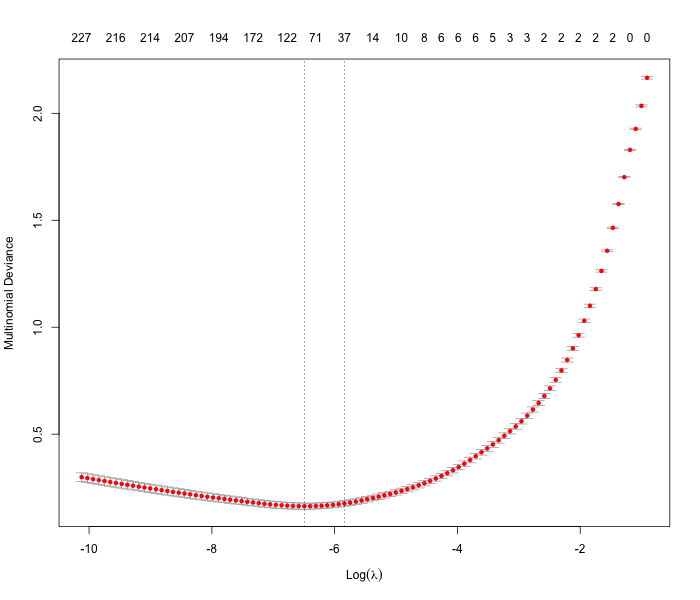
\includegraphics[width=0.5\linewidth,height=\textheight,keepaspectratio]{image/clf0-plot.png}

\textsubscript{Source:
\href{https://h-christy.github.io/data-ethics-final/index.qmd.html}{Article
Notebook}}

\begin{verbatim}
[1] 0.9902837
\end{verbatim}

\textsubscript{Source:
\href{https://h-christy.github.io/data-ethics-final/index.qmd.html}{Article
Notebook}}

\begin{verbatim}
[1] 0.989899
\end{verbatim}

\textsubscript{Source:
\href{https://h-christy.github.io/data-ethics-final/index.qmd.html}{Article
Notebook}}

\begin{verbatim}
Confusion Matrix and Statistics

               Reference
Prediction      more tolerant in between less tolerant
  more tolerant           400          4             3
  in between                0        511             3
  less tolerant             1          2           363

Overall Statistics
                                          
               Accuracy : 0.9899          
                 95% CI : (0.9828, 0.9946)
    No Information Rate : 0.4017          
    P-Value [Acc > NIR] : <2e-16          
                                          
                  Kappa : 0.9847          
                                          
 Mcnemar's Test P-Value : 0.1577          

Statistics by Class:

                     Class: more tolerant Class: in between
Sensitivity                        0.9975            0.9884
Specificity                        0.9921            0.9961
Pos Pred Value                     0.9828            0.9942
Neg Pred Value                     0.9989            0.9922
Prevalence                         0.3116            0.4017
Detection Rate                     0.3108            0.3970
Detection Prevalence               0.3162            0.3994
Balanced Accuracy                  0.9948            0.9922
                     Class: less tolerant
Sensitivity                        0.9837
Specificity                        0.9967
Pos Pred Value                     0.9918
Neg Pred Value                     0.9935
Prevalence                         0.2867
Detection Rate                     0.2821
Detection Prevalence               0.2844
Balanced Accuracy                  0.9902
\end{verbatim}

\textsubscript{Source:
\href{https://h-christy.github.io/data-ethics-final/index.qmd.html}{Article
Notebook}}

\textsubscript{Source:
\href{https://h-christy.github.io/data-ethics-final/index.qmd.html}{Article
Notebook}}

\textsubscript{Source:
\href{https://h-christy.github.io/data-ethics-final/index.qmd.html}{Article
Notebook}}

\begin{longtable}[]{@{}lr@{}}
\toprule\noalign{}
predictor & n \\
\midrule\noalign{}
\endhead
\bottomrule\noalign{}
\endlastfoot
(Intercept) & 3 \\
admitted\_communist\_allow\_speak5 & 2 \\
admitted\_communist\_buy\_soap5 & 2 \\
admitted\_communist\_put\_jail5 & 2 \\
alledged\_communist\_fire\_teacher5 & 2 \\
censor\_antireligion\_book5 & 2 \\
censor\_antireligion\_speaker5 & 2 \\
censor\_antireligion\_speaker8 & 2 \\
censor\_socialist\_book5 & 2 \\
censor\_socialist\_speaker8 & 2 \\
many\_communists\_defense\_plants8 & 2 \\
many\_communists\_us5 & 2 \\
\end{longtable}

\textsubscript{Source:
\href{https://h-christy.github.io/data-ethics-final/index.qmd.html}{Article
Notebook}}

\textsubscript{Source:
\href{https://h-christy.github.io/data-ethics-final/index.qmd.html}{Article
Notebook}}

\subsubsection{\texorpdfstring{3-class classification:
\texttt{tolerance\_broader} based on the measure with wiggle
room}{3-class classification: tolerance\_broader based on the measure with wiggle room}}\label{class-classification-tolerance_broader-based-on-the-measure-with-wiggle-room}

\textsubscript{Source:
\href{https://h-christy.github.io/data-ethics-final/index.qmd.html}{Article
Notebook}}

\textsubscript{Source:
\href{https://h-christy.github.io/data-ethics-final/index.qmd.html}{Article
Notebook}}

\textsubscript{Source:
\href{https://h-christy.github.io/data-ethics-final/index.qmd.html}{Article
Notebook}}

\textsubscript{Source:
\href{https://h-christy.github.io/data-ethics-final/index.qmd.html}{Article
Notebook}}

\textsubscript{Source:
\href{https://h-christy.github.io/data-ethics-final/index.qmd.html}{Article
Notebook}}

\textsubscript{Source:
\href{https://h-christy.github.io/data-ethics-final/index.qmd.html}{Article
Notebook}}

\begin{Shaded}
\begin{Highlighting}[]
\NormalTok{clf }\OtherTok{\textless{}{-}} \FunctionTok{cv.glmnet}\NormalTok{(}
\NormalTok{  x\_train, y\_train,}\AttributeTok{family =} \StringTok{"multinomial"}\NormalTok{,}
  \AttributeTok{alpha =} \DecValTok{1}\NormalTok{, }\AttributeTok{type.multinomial =} \StringTok{"ungrouped"}
\NormalTok{)}
\CommentTok{\# png("clf{-}plot.png", width = 700, height = 600)}
\CommentTok{\# plot(clf)}
\CommentTok{\# dev.off()}
\NormalTok{lambda\_best }\OtherTok{\textless{}{-}}\NormalTok{ clf}\SpecialCharTok{$}\NormalTok{lambda}\FloatTok{.1}\NormalTok{se}
\CommentTok{\# 0.00391}
\NormalTok{lambda\_seq }\OtherTok{\textless{}{-}}\NormalTok{ clf}\SpecialCharTok{$}\NormalTok{lambda}
\CommentTok{\# saveRDS(lambda\_seq, file = "data/clf{-}lambda{-}seq.rds")}
\end{Highlighting}
\end{Shaded}

\pandocbounded{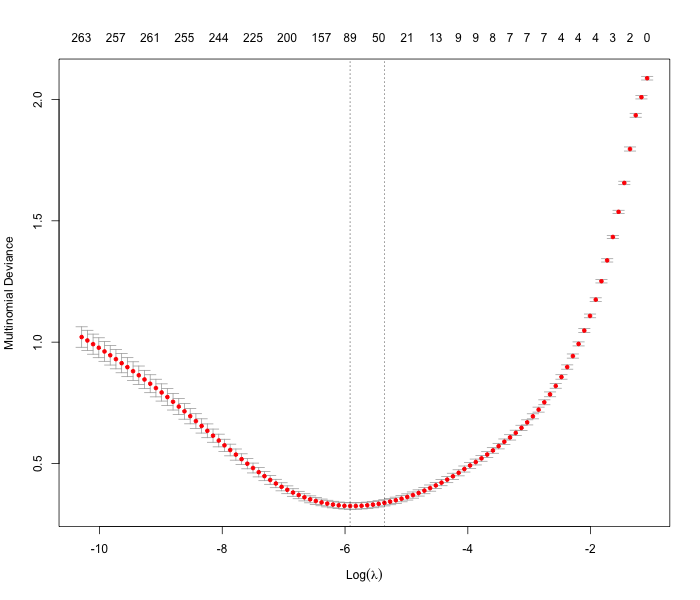
\includegraphics[keepaspectratio]{image/clf-plot.png}}

\textsubscript{Source:
\href{https://h-christy.github.io/data-ethics-final/index.qmd.html}{Article
Notebook}}

\begin{verbatim}
[1] 0.958803
\end{verbatim}

\textsubscript{Source:
\href{https://h-christy.github.io/data-ethics-final/index.qmd.html}{Article
Notebook}}

\begin{verbatim}
[1] 0.950272
\end{verbatim}

\textsubscript{Source:
\href{https://h-christy.github.io/data-ethics-final/index.qmd.html}{Article
Notebook}}

\begin{verbatim}
Confusion Matrix and Statistics

               Reference
Prediction      more tolerant in between less tolerant
  more tolerant           505          4             5
  in between                9        489            12
  less tolerant             7         27           229

Overall Statistics
                                          
               Accuracy : 0.9503          
                 95% CI : (0.9369, 0.9615)
    No Information Rate : 0.4048          
    P-Value [Acc > NIR] : < 2e-16         
                                          
                  Kappa : 0.9222          
                                          
 Mcnemar's Test P-Value : 0.04548         

Statistics by Class:

                     Class: more tolerant Class: in between
Sensitivity                        0.9693            0.9404
Specificity                        0.9883            0.9726
Pos Pred Value                     0.9825            0.9588
Neg Pred Value                     0.9793            0.9601
Prevalence                         0.4048            0.4040
Detection Rate                     0.3924            0.3800
Detection Prevalence               0.3994            0.3963
Balanced Accuracy                  0.9788            0.9565
                     Class: less tolerant
Sensitivity                        0.9309
Specificity                        0.9673
Pos Pred Value                     0.8707
Neg Pred Value                     0.9834
Prevalence                         0.1911
Detection Rate                     0.1779
Detection Prevalence               0.2044
Balanced Accuracy                  0.9491
\end{verbatim}

\textsubscript{Source:
\href{https://h-christy.github.io/data-ethics-final/index.qmd.html}{Article
Notebook}}

\textsubscript{Source:
\href{https://h-christy.github.io/data-ethics-final/index.qmd.html}{Article
Notebook}}

\textsubscript{Source:
\href{https://h-christy.github.io/data-ethics-final/index.qmd.html}{Article
Notebook}}

\begin{longtable}[]{@{}lr@{}}
\toprule\noalign{}
predictor & n \\
\midrule\noalign{}
\endhead
\bottomrule\noalign{}
\endlastfoot
(Intercept) & 3 \\
admitted\_communist\_allow\_speak5 & 2 \\
admitted\_communist\_buy\_soap5 & 2 \\
admitted\_communist\_put\_jail5 & 2 \\
admitted\_communist\_remove\_book\_library5 & 2 \\
alledged\_communist\_fire\_clerk5 & 2 \\
alledged\_communist\_fire\_clerk8 & 2 \\
alledged\_communist\_fire\_defense\_plant5 & 2 \\
alledged\_communist\_fire\_high\_school\_teacher5 & 2 \\
alledged\_communist\_fire\_singer5 & 2 \\
alledged\_communist\_fire\_teacher5 & 2 \\
alledged\_communist\_make\_community\_speech5 & 2 \\
\end{longtable}

\textsubscript{Source:
\href{https://h-christy.github.io/data-ethics-final/index.qmd.html}{Article
Notebook}}

\subsubsection{Are these selected Items capturing most of the
variances?}\label{are-these-selected-items-capturing-most-of-the-variances}

\textsubscript{Source:
\href{https://h-christy.github.io/data-ethics-final/index.qmd.html}{Article
Notebook}}

\textsubscript{Source:
\href{https://h-christy.github.io/data-ethics-final/index.qmd.html}{Article
Notebook}}

\textsubscript{Source:
\href{https://h-christy.github.io/data-ethics-final/index.qmd.html}{Article
Notebook}}

\subsubsection{Learning: Predicting Tolerance Score without the original
15
items}\label{learning-predicting-tolerance-score-without-the-original-15-items}

\textsubscript{Source:
\href{https://h-christy.github.io/data-ethics-final/index.qmd.html}{Article
Notebook}}

\textsubscript{Source:
\href{https://h-christy.github.io/data-ethics-final/index.qmd.html}{Article
Notebook}}

\textsubscript{Source:
\href{https://h-christy.github.io/data-ethics-final/index.qmd.html}{Article
Notebook}}

\textsubscript{Source:
\href{https://h-christy.github.io/data-ethics-final/index.qmd.html}{Article
Notebook}}

\begin{longtable}[]{@{}lr@{}}
\toprule\noalign{}
tolerance\_broader0 & n \\
\midrule\noalign{}
\endhead
\bottomrule\noalign{}
\endlastfoot
in between & 426 \\
less tolerant & 261 \\
more tolerant & 813 \\
\end{longtable}

\textsubscript{Source:
\href{https://h-christy.github.io/data-ethics-final/index.qmd.html}{Article
Notebook}}

\textsubscript{Source:
\href{https://h-christy.github.io/data-ethics-final/index.qmd.html}{Article
Notebook}}

\textsubscript{Source:
\href{https://h-christy.github.io/data-ethics-final/index.qmd.html}{Article
Notebook}}

\textsubscript{Source:
\href{https://h-christy.github.io/data-ethics-final/index.qmd.html}{Article
Notebook}}

\textsubscript{Source:
\href{https://h-christy.github.io/data-ethics-final/index.qmd.html}{Article
Notebook}}

\textsubscript{Source:
\href{https://h-christy.github.io/data-ethics-final/index.qmd.html}{Article
Notebook}}

\begin{Shaded}
\begin{Highlighting}[]
\NormalTok{clf3 }\OtherTok{\textless{}{-}} \FunctionTok{cv.glmnet}\NormalTok{(}
\NormalTok{  x\_train, y\_train, }\AttributeTok{family =} \StringTok{"multinomial"}\NormalTok{,}
  \AttributeTok{alpha =} \FloatTok{0.75}\NormalTok{, }\AttributeTok{type.multinomial =} \StringTok{"ungrouped"}
\NormalTok{)}
\NormalTok{lambda\_1se3 }\OtherTok{\textless{}{-}}\NormalTok{ clf3}\SpecialCharTok{$}\NormalTok{lambda}\FloatTok{.1}\NormalTok{se}
\NormalTok{lambda\_1se3}
\CommentTok{\# 0.01726083}
\NormalTok{lambda\_seq3 }\OtherTok{\textless{}{-}}\NormalTok{ clf3}\SpecialCharTok{$}\NormalTok{lambda}
\CommentTok{\# saveRDS(lambda\_seq3, file = "data/clf3{-}lambda{-}seq.rds")}

\CommentTok{\# png("image/clf3{-}plot.png", width = 700, height = 600)}
\CommentTok{\# plot(clf3)}
\CommentTok{\# dev.off()}
\end{Highlighting}
\end{Shaded}

\pandocbounded{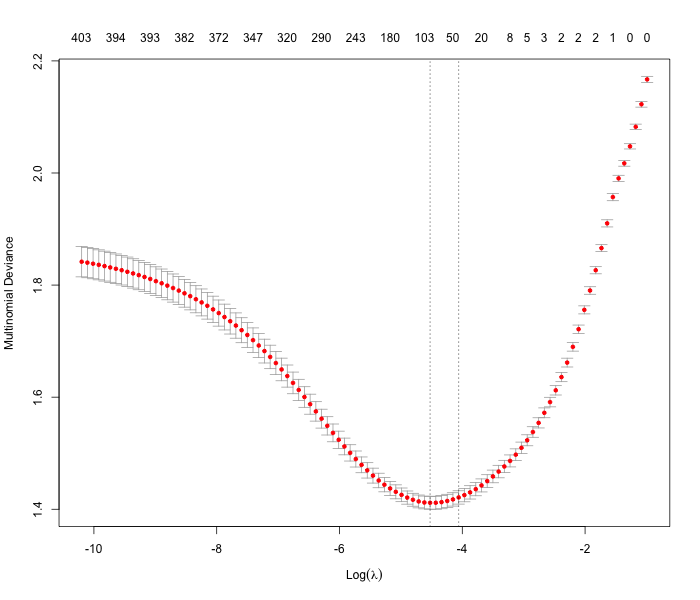
\includegraphics[keepaspectratio]{image/clf3-plot.png}}

\textsubscript{Source:
\href{https://h-christy.github.io/data-ethics-final/index.qmd.html}{Article
Notebook}}

\begin{verbatim}
[1] 0.7188107
\end{verbatim}

\textsubscript{Source:
\href{https://h-christy.github.io/data-ethics-final/index.qmd.html}{Article
Notebook}}

\begin{verbatim}
[1] 0.6985237
\end{verbatim}

\textsubscript{Source:
\href{https://h-christy.github.io/data-ethics-final/index.qmd.html}{Article
Notebook}}

\begin{verbatim}
Confusion Matrix and Statistics

               Reference
Prediction      more tolerant in between less tolerant
  more tolerant           264         65            39
  in between              125        435           130
  less tolerant            12         17           200

Overall Statistics
                                          
               Accuracy : 0.6985          
                 95% CI : (0.6726, 0.7235)
    No Information Rate : 0.4017          
    P-Value [Acc > NIR] : < 2.2e-16       
                                          
                  Kappa : 0.5322          
                                          
 Mcnemar's Test P-Value : < 2.2e-16       

Statistics by Class:

                     Class: more tolerant Class: in between
Sensitivity                        0.6584            0.8414
Specificity                        0.8826            0.6688
Pos Pred Value                     0.7174            0.6304
Neg Pred Value                     0.8509            0.8626
Prevalence                         0.3116            0.4017
Detection Rate                     0.2051            0.3380
Detection Prevalence               0.2859            0.5361
Balanced Accuracy                  0.7705            0.7551
                     Class: less tolerant
Sensitivity                        0.5420
Specificity                        0.9684
Pos Pred Value                     0.8734
Neg Pred Value                     0.8403
Prevalence                         0.2867
Detection Rate                     0.1554
Detection Prevalence               0.1779
Balanced Accuracy                  0.7552
\end{verbatim}

\textsubscript{Source:
\href{https://h-christy.github.io/data-ethics-final/index.qmd.html}{Article
Notebook}}

\subsubsection{Acquired the class specific variables and their
coefficients}\label{acquired-the-class-specific-variables-and-their-coefficients}

\textsubscript{Source:
\href{https://h-christy.github.io/data-ethics-final/index.qmd.html}{Article
Notebook}}

\textsubscript{Source:
\href{https://h-christy.github.io/data-ethics-final/index.qmd.html}{Article
Notebook}}

\begin{longtable}[]{@{}lr@{}}
\toprule\noalign{}
predictor & n \\
\midrule\noalign{}
\endhead
\bottomrule\noalign{}
\endlastfoot
(Intercept) & 3 \\
admitted\_communist\_fire\_clerk5 & 2 \\
admitted\_communist\_lose\_citizenship5 & 2 \\
break\_friendship\_former\_communist5 & 2 \\
censor\_antireligion\_teacher5 & 2 \\
child\_rearing\_respect3 & 2 \\
last\_grade\_finished\_school5 & 2 \\
remember\_hiss\_caught8 & 2 \\
admitted\_communist\_fire\_college\_professor5 & 1 \\
admitted\_communist\_lose\_citizenship8 & 1 \\
alledged\_communist\_buy\_soap5 & 1 \\
alledged\_communist\_fire\_singer5 & 1 \\
\end{longtable}

\textsubscript{Source:
\href{https://h-christy.github.io/data-ethics-final/index.qmd.html}{Article
Notebook}}

\subsubsection{Worrying about Internal Communist
Threats}\label{worrying-about-internal-communist-threats}

\begin{verbatim}

    Pearson's Chi-squared test

data:  toler_rigid_tb
X-squared = 491.09, df = 10, p-value < 2.2e-16
\end{verbatim}

\textsubscript{Source:
\href{https://h-christy.github.io/data-ethics-final/index.qmd.html}{Article
Notebook}}

\begin{verbatim}
            
                  agree   disagree  dont know
  tolerance0  3.6776281 -5.3964437  1.1128421
  tolerance1 -2.3955483 -1.0211719 10.7874512
  tolerance2  4.5040579 -6.1915000  0.3030713
  tolerance3  2.7420911 -2.5744267 -2.8481376
  tolerance4 -0.6175252  2.2641002 -3.6331099
  tolerance5 -7.2561266 11.9240239 -5.4354457
\end{verbatim}

\textsubscript{Source:
\href{https://h-christy.github.io/data-ethics-final/index.qmd.html}{Article
Notebook}}

\begin{verbatim}

    Pearson's Chi-squared test

data:  toler_danger_tb
X-squared = 410.67, df = 25, p-value < 2.2e-16
\end{verbatim}

\textsubscript{Source:
\href{https://h-christy.github.io/data-ethics-final/index.qmd.html}{Article
Notebook}}

\begin{verbatim}
            
                  danger0      danger1      danger2      danger3      danger4
  tolerance0 -2.970715176 -2.658964979 -2.459910036  0.974739884  2.152232514
  tolerance1 -4.609232171 -1.006527133  4.547776892 -1.482352369  0.006717332
  tolerance2 -3.631408736 -5.657972356  0.475321324  2.009535358  1.330107400
  tolerance3 -0.858497500 -0.790142288 -1.598983893  2.256620306  1.165660786
  tolerance4  0.394465523  0.926642029 -0.167803951  0.370962087 -0.093407449
  tolerance5 10.328080755  8.630383914 -1.058231155 -3.774441827 -3.913075010
            
                  danger5
  tolerance0  4.929822736
  tolerance1 -0.973974888
  tolerance2  3.228408105
  tolerance3 -0.075048875
  tolerance4 -1.188784303
  tolerance5 -5.126832308
\end{verbatim}

\textsubscript{Source:
\href{https://h-christy.github.io/data-ethics-final/index.qmd.html}{Article
Notebook}}

\textsubscript{Source:
\href{https://h-christy.github.io/data-ethics-final/index.qmd.html}{Article
Notebook}}

\pandocbounded{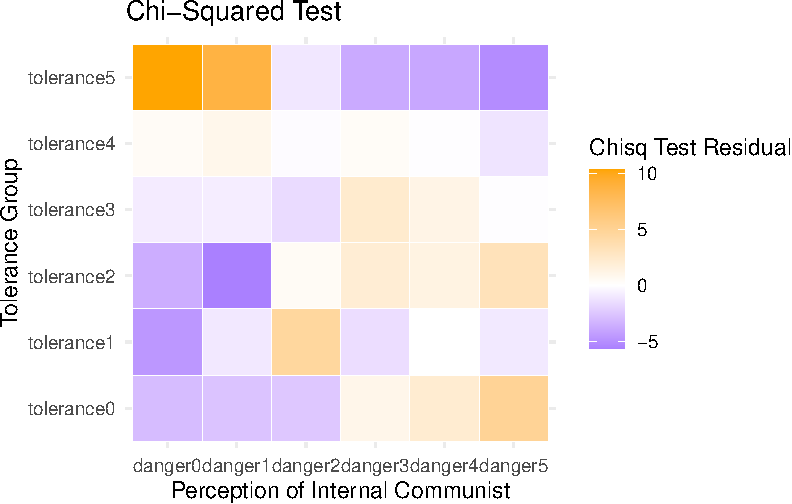
\includegraphics[keepaspectratio]{index_files/figure-pdf/unnamed-chunk-85-1.pdf}}

\textsubscript{Source:
\href{https://h-christy.github.io/data-ethics-final/index.qmd.html}{Article
Notebook}}

\subsection{Results}\label{results}

\subsubsection{Reflections}\label{reflections}

\subsection*{Policy Recommendation}\label{policy-recommendation}
\addcontentsline{toc}{subsection}{Policy Recommendation}

\phantomsection\label{refs}
\begin{CSLReferences}{1}{0}
\bibitem[\citeproctext]{ref-fundfortherepublicCommunismConformityAmp2020}
Fund For The Republic, and Samuel A. Stouffer. 2020. {``Communism,
{Conformity} \&Amp; {Civil Liberties}.''} Roper Center for Public
Opinion Research. \url{https://doi.org/10.25940/ROPER-31089514}.

\bibitem[\citeproctext]{ref-stoufferCommunismConformityCivil1992}
Stouffer, Samuel A. 1992. {``Communism, {Conformity}, and {Civil
Liberties Study}, 1954.''} {Inter-university Consortium for Political
and Social Research}. \url{https://doi.org/10.3886/ICPSR07202.v2}.

\bibitem[\citeproctext]{ref-stoufferTechniqueImprovingCumulative1952}
STOUFFER, SAMUEL A., EDGAR F. BORGATTA, DAVID G. HAYS, and ANDREW F.
HENRY. 1952. {``A {Technique} for {Improving Cumulative Scales}*.''}
\emph{Public Opinion Quarterly} 16 (2): 273--91.
\url{https://doi.org/10.1086/266388}.

\bibitem[\citeproctext]{ref-stouffer1955communism}
Stouffer, Samuel Andrew. 1955. \emph{Communism, Conformity, and Civil
Liberties: {A} Cross-Section of the Nation Speaks Its Mind}. Transaction
Publishers.

\bibitem[\citeproctext]{ref-tesslerSocialScienceResearch2022}
Tessler, Mark. 2022. \emph{Social {Science Research} in the {Arab World}
and {Beyond}: {A Guide} for {Students}, {Instructors} and
{Researchers}}. Springer Nature.

\end{CSLReferences}




\end{document}
